% !TEX root = ../main.tex
\pagebreak[0]
\section{Introduction}\label{sec:introduction}
\subsection{Rupert's property}\label{subsec:ruperts-property}

Can a cube pass through a hole in another cube of the same size?
The earliest known written account of this problem is by
\citet[pp.~470--471]{Wallis1693}, who records that Prince Rupert of the Rhine
wagered that it could. Wallis gave a geometric
solution to this apparently
impossible puzzle: suitably orienting the two cubes allows one to slide,
without turning, through a straight tunnel cut in the other, with positive
clearance. Thus the cube has \emph{Rupert's property}, or, equivalently,
the cube is \emph{Rupert}.
We call the moving body the \emph{plug} and the body through which it moves
the \emph{hole}.

It turns out that even a somewhat larger cube can pass through. The limiting
ratio of the plug's edge length to the hole's is
\[
  \frac{3\sqrt{2}}{4} \approx 1.060660172.
\]
The construction giving this ratio was found by Pieter Nieuwland and
published posthumously by \citet[pp.~608--610]{VanSwinden1816}.
Its optimality when the plug moves along a straight line without
turning was proved by
\citet{BezdekEtAl2021}. This limiting scale factor is called the cube's
\emph{Nieuwland number}; the same notion applies to other polyhedra.

\begin{figure}[htbp]
\centering
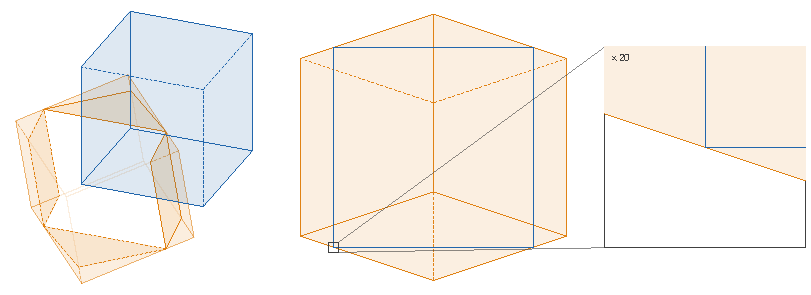
\includegraphics[width=0.85\linewidth]{figures/nieuwland-cube}
\caption{Nieuwland's passage for the cube. Left: \fc{Hole}{a unit cube (orange, faint)} with the tunnel cut out along the direction $(2,2,-1)$, and \fc{Plug}{a cube of edge $3\sqrt2/4$ (blue)} leaving it; only four wedges of the unit cube remain. Middle: both shadows along the direction of motion, a \fc{Plug}{square} inside a \fc{Hole}{hexagon}, \fc{Hole}{the hole's shadow tinted}. Right: a corner of the square, enlarged: it lies on the boundary of the hexagon, so no larger cube passes. In this and the later drawings, in space and in projection, the edges on the far side of each solid are dashed.}
\label{fig:nieuwland-cube}
\end{figure}

The same question applies to any convex polyhedron: can a congruent plug
pass through it in this way? \citet{JerrardWetzelYuan2017}
suggested that every convex polyhedron might be Rupert, and
\citet{ChaiYuanZamfirescu2018} stated this as a conjecture the following year.
A few years later, \citet{SteiningerYurkevich2023} conjectured that the
rhombicosidodecahedron (RID), a highly regular and symmetric Archimedean
solid with 60 vertices, was an exception. A polyhedron without Rupert's property is called \emph{Nopert}, a term
coined by Tom Murphy VII, also known as Tom~7, combining \emph{Nope} and
\emph{Rupert} \citep[p.~352]{Murphy2025}.
\citet{SteiningerYurkevichNopertV2} subsequently constructed the first convex polyhedron
proved to be Nopert, the \emph{Noperthedron}, but their proof did not settle
the RID \citep[Section~9.1]{SteiningerYurkevichNopertV2}.
Here we settle the RID's case with new geometric arguments that handle
its exotic cases.

\begin{theorem}\label{thm:main}
  The rhombicosidodecahedron is Nopert.
\end{theorem}

We call a choice of the plug's and hole's orientations, their relative displacement
and the direction of motion a \emph{configuration}.
The proof is computer-assisted. We divide the configuration space into
$192{,}696$ regions, each resolved using exact arithmetic calculations.
The final argument is given in
\cref{subsec:complete-coverage-and-the-main-theorem}.

\paragraph{The key idea.}
Most configurations are easy to rule out: some vertex of the plug sticks
out of the tunnel, and it still does after any small change of the
configuration, so a whole region around the configuration can be
eliminated at once. The obstacle is formed by the configurations in which
the plug touches the walls of the tunnel without sticking out. The
simplest example is a plug turned exactly like the hole: the two copies
then line up, and so do their shadows. Every strict inequality that could
exclude a fit vanishes at such a configuration, so no region containing
it can be eliminated by testing inequalities, however finely the regions
are subdivided. Yet the plug does stick out once it is turned slightly.
Suppose, for instance, that turning it by a small angle $x\ge0$ moves some
vertex outward by the amount $p(x,y)=x(1+x-y)$, where $y\in[0,1/2]$ stands
for the viewing direction. A sign test of $p$ must fail on any region
containing $x=0$, where $p$ vanishes. The factor $x$, however, is explicit:
the quotient $p/x=1+x-y$ is at least $1/2$ throughout, one sign test shows
it, and the configurations with $x=0$ are already known not to be fits.

We turn this observation into a single lemma, the \emph{zoom lemma}
(\cref{lem:zoom-lemma}). Around a set of configurations known to contain
no fit, a \emph{zoom} is a polynomial change of coordinates that
magnifies the neighbourhood of that set, so that the distance from it
becomes a coordinate that can be divided out exactly. After the division,
one exact sign test settles a whole region, including the touching
configurations themselves. The Local and Exotic components are instances of
this lemma, whose zooms differ only in the set around which they magnify
and in how many distances they divide out; the Domain and Global tests are
the same idea with nothing divided out. The four \emph{components} of the
proof, each a method for eliminating whole regions of configurations, are
listed in \cref{tab:components}.

\begin{table}[htbp]
\centering
\small
\begin{tabular}{llll}
  \toprule
  Component & Eliminates regions & Divides out & Section\\
  \midrule
  Domain & outside the symmetry-reduced domain & nothing & \ref{subsec:domain-component-skipping-boxes-outside-the-reduced-domain}\\
  Global & where some plug vertex sticks out & nothing & \ref{sec:global-component}\\
  Local & around the plug turned like the hole & the size of the rotation & \ref{sec:local-component}\\
  Exotic & around the other touching configurations & one or two distances & \ref{sec:square-and-pentagon-configurations}--\ref{sec:endpoint-and-crossing-configurations}\\
  \bottomrule
\end{tabular}
\caption{The four components of the proof.}
\label{tab:components}
\end{table}

\subsection{Previous approaches and the remaining difficulty}\label{subsec:previous-approaches-and-the-remaining-difficulty}

When the plug can pass through the hole with positive clearance, we call
this a \emph{fit} configuration.
To prove that a polyhedron is Rupert, even a single fit configuration is
enough, though finding one can be difficult. Examples include the
construction of \citet{Fredriksson2024} for the triakis tetrahedron and
the proof of \citet{RenshawRupertLean} in the Lean proof assistant that
Tom~7's candidate~\#214 is Rupert.
However, to prove that a polyhedron is Nopert, we must rule out every
possible fit configuration across the entire continuous space of
orientations, displacements and directions of motion. An unsuccessful
search over finitely many configurations, such as those sampled by the
randomized algorithms of \citet{SteiningerYurkevich2023}, however extensive,
is insufficient to rule out all infinitely many configurations.

\begin{figure}[htbp]
\centering
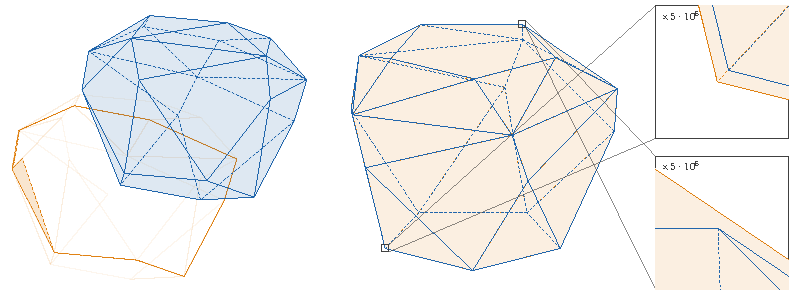
\includegraphics[width=0.85\linewidth]{figures/nopert214}
\caption{Tom~7's candidate~\#214 passes through itself, in the configuration of \citet{RenshawRupertLean}. Left: the tunnel removes all of \fc{Hole}{the hole (orange)} but a thin rim; \fc{Plug}{the plug (blue)} leaves it. Middle: the two shadows, indistinguishable at this scale. Right: the two places of least clearance, enlarged five million times; the gap is about $1.8\cdot10^{-8}$, for a solid of circumradius~$1$.}
\label{fig:nopert214}
\end{figure}

\paragraph{Constructive results and numerical searches.}
\citet{JerrardWetzelYuan2017} completed the proof that all five Platonic
solids are Rupert, building on earlier results for the cube, tetrahedron
and octahedron.
\begin{figure}[htbp]
\centering
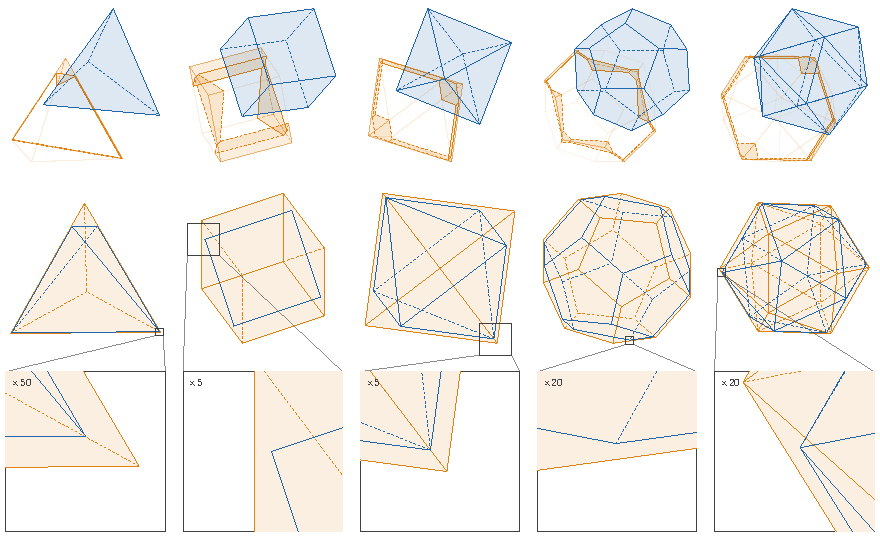
\includegraphics[width=0.95\linewidth]{figures/platonic}
\caption{Passages of the tetrahedron, cube, octahedron, dodecahedron and icosahedron, found by a numerical search. Top: \fc{Hole}{the hole (orange, faint)} with the tunnel cut out, and \fc{Plug}{the plug (blue)} leaving it. Middle: the shadows along the direction of motion. Bottom: the place of least clearance, enlarged. The plugs could be enlarged by factors of about $1.0145$, $1.0607$, $1.0607$, $1.0108$ and $1.0108$ and still pass; only the tetrahedron, which is not centrally symmetric, needs its plug's shadow shifted.}
\label{fig:platonic}
\end{figure}
\citet{ChaiYuanZamfirescu2018} examined the Archimedean solids and proved
Rupertness for eight of the thirteen. Subsequent work brought the total to
ten, leaving the snub cube, the RID and the snub dodecahedron unresolved
at that stage \citep{SteiningerYurkevich2023}.

Computational methods enabled more extensive searches for fit
configurations. \citet{SteiningerYurkevich2023} developed randomized searches
for such configurations and improved lower bounds for Nieuwland numbers
by perturbing known examples. \citet{Fredriksson2024} used nonlinear
optimization of the viewing directions from many starting points, and
\citet{GosainGrimmer2025V1} combined nonsmooth local optimization with
high-precision calculations of scale factors.

The triakis tetrahedron, a Catalan solid with eight vertices,
illustrates how a fit configuration can escape a large search.
It was among the solids left unresolved by \citet{SteiningerYurkevich2023}
in their randomized searches.
\citet{Fredriksson2024} then found a configuration giving a reported lower bound of
$1.000004$ for its Nieuwland number, corresponding to a clearance of only
about four parts per million in linear scale.
This shows how little room a fit configuration may have and gives
a concrete example of a configuration missed by earlier randomized searches.
More extensive searches and higher numerical precision can improve the
chances of finding such configurations, but failure to find one still does
not prove nonexistence.

\begin{figure}[htbp]
\centering
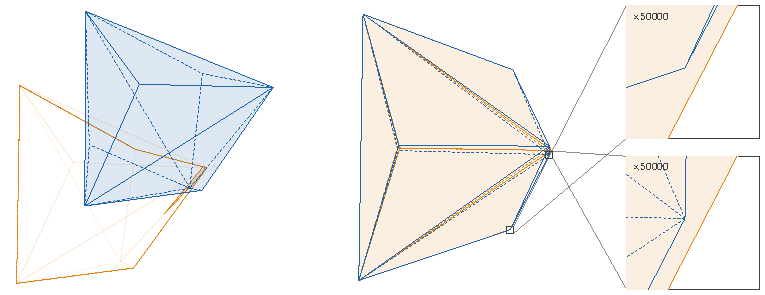
\includegraphics[width=0.82\linewidth]{figures/triakis}
\caption{The triakis tetrahedron passes through itself \citep{Fredriksson2024}. Drawn as in \cref{fig:nopert214}, with the two places of least clearance enlarged $50{,}000$ times; the gap is about $3.3\cdot10^{-6}$ at circumradius $5\sqrt6/8\approx1.53$. The parameters are Fredriksson's, refined slightly by a local numerical minimisation that changes none of them by more than $2.3\cdot10^{-5}$.}
\label{fig:triakis}
\end{figure}

\paragraph{Proving non-Rupertness.}
\citet{SteiningerYurkevichNopertV2} prove that the Noperthedron is Nopert
by combining arguments eliminating whole regions of configurations with
special treatment of boundary cases. They also explain why their local
theorem is insufficient for the RID, identifying an exotic viewing
direction and stating that its neighbourhood can be treated using
polynomial inequalities, while
reporting further difficult regions
\citep[Section~9.1]{SteiningerYurkevichNopertV2}.

The RID was a promising candidate for this research because of its highly
regular structure and many
symmetries, including central symmetry: reflecting it through its centre
leaves the RID unchanged. Central symmetry also simplifies the problem,
as explained in \cref{subsec:projection-containment}.
For such a regular solid, an extremely narrow, overlooked region of
fit configurations seemed less plausible to us. Despite this
intuition, we needed a way to recognise and rigorously verify a fit
configuration if one existed contrary to our expectations. We explain
how to handle this possibility in \cref{subsec:robustly-detecting-potential-rupertness}.

\citet{SteiningerYurkevich2023} also give an algorithm guaranteed to decide
whether a polyhedron with algebraic coordinates is Rupert, which they
describe as too computationally expensive for practical use.
Our aim is a feasible computer-assisted proof for the RID that addresses
the special configurations where ordinary elimination methods break down.

\subsection{Overview of the proof}\label{subsec:overview-of-the-proof}

For \emph{translative motion}, meaning motion without turning, the problem
has a useful two-dimensional description.
Project the plug and hole perpendicularly onto a plane normal to the direction
of motion, viewing their projections as filled \emph{shadows}. A fit configuration
is one in which the plug's shadow lies entirely in the interior of the hole's shadow.
For centrally symmetric convex bodies, relative translations can be removed:
if any relative displacement gives fit, coincident projected centres give
fit as well \citep{SteiningerYurkevich2023}. We give the argument in
\cref{subsec:projection-containment} so that this reduction requires no
background from the Rupert literature.

We may then fix the hole and describe a configuration by two parameters for
the viewing direction and three for the plug's relative rotation.
Our coordinates make the relevant expressions rational functions of these
five parameters. Clearing denominators of known positive sign reduces the
comparisons to polynomial inequalities. In contrast, the angular
parametrisation in the Noperthedron proof of
\citet[Section~6.1]{SteiningerYurkevichNopertV2} requires rigorously bounded
approximations to sine and cosine.
The RID's symmetries allow us to restrict attention to a small bounded
region of these coordinates while retaining at least one representative of
every remaining configuration. The parametrisation and the proof that these
representatives suffice are developed in
\cref{sec:geometric-formulation,sec:symmetry-reduced-domain}.

\paragraph{Eliminating configuration regions.}
Within that region, the procedure attempts to eliminate an entire parameter
region at once. Only representatives in the symmetry-reduced domain need to
be eliminated; regions entirely outside it can be skipped.
We call each method for certifying such an elimination a \emph{component}.
When no available component succeeds, the region is bisected
and both halves are retained for further examination. Failure of a test is
inconclusive: it neither establishes a fit configuration nor gives a reason
to discard the region. Together, the eliminated regions and their checked
reasons form a \emph{certificate}. \Cref{sec:branch-and-bound-elimination-in-the-reduced-domain}
explains the subdivision and what is required of such a certificate;
the exact calculations behind the checks are developed in
\cref{sec:reduction-to-exact-arithmetic}.

\paragraph{Completing the certificate.}
The remaining difficulty is to make subdivision terminate with a complete
certificate. We develop components successively to handle configurations
that the preceding ones leave unresolved.
First, if part of the plug's shadow protrudes beyond the hole's shadow,
we call this a \emph{poke} configuration. A sufficiently small change
preserves that protrusion, allowing us to eliminate a whole surrounding
region. The \emph{Global} component of \cref{sec:global-component}
eliminates these cases.

The difficulty arises when the plug's shadow is contained in the hole's,
but their boundaries meet: we call this a \emph{touch} configuration.
For example, in \emph{aligned configurations}, the plug and hole have the
same physical orientation, allowing for the RID's symmetries. The centred
bodies then coincide, as do their shadows. There is no protrusion to detect.
Further subdivision leaves at least one region containing the same touch
configuration, so testing for protrusion alone cannot complete the elimination.
We give formal definitions of fit, touch and poke in
\cref{subsec:the-margin-function-and-fit-poke-touch}.

Around aligned configurations, we instead study how the plug's vertices
move when the plug begins to rotate. The inequality expressing outward
motion contains the size of the rotation as an explicit factor, which
vanishes exactly at the aligned configurations, as in the example above.
\Cref{sec:local-component} develops the \emph{Local} component from this
observation and states the zoom lemma in general
(\cref{subsec:the-zoom-lemma}).
At two exotic viewing directions, the outward motion itself vanishes
to first order, and \cref{sec:square-and-pentagon-configurations} divides
out a second distance there.

Surprisingly, even after the aligned configurations have been
handled, non-aligned touch configurations remain---what
seems to us to be a rare feature of the RID\@. These families lie in two
planes of configurations that contain no fit, because in one direction the
plug reaches exactly as far as the hole. The same lemma, now dividing by
the distance from these planes, handles them, again with two distances at
the end of one family and where the two families cross
(\cref{sec:arc-configurations,sec:endpoint-and-crossing-configurations}).
These covers, together with those of
\cref{sec:square-and-pentagon-configurations}, form the \emph{Exotic}
component. With it, the collection of four components eliminates the
entire symmetry-reduced configuration space.

All accepted inequalities are checked with exact arithmetic. The final
certificate records a reason for each eliminated region. Its verification has
two distinct tasks: check that every reason is valid for all required
configurations in its region, and check that the regions together cover
all those configurations.
Together these establish \cref{thm:main}. We unify these requirements and
describe the implementation and computation details in
\cref{sec:generating-and-verifying-the-certificate}.
